\documentclass[12pt]{article}

\usepackage[margin=1in]{geometry}
\usepackage{graphicx}
    \graphicspath{{../media/}} 
\usepackage{float}

\setlength{\parskip}{1em}
\setlength{\parindent}{0em}

\renewcommand\thesection{\hspace{-1em}}
\renewcommand\thesubsection{\hspace{-1em}}

\title{Criterion B - Planning}
\author{}
\date{}

\begin{document}
\maketitle

\section{Flowchart}
%
\begin{figure}[H]
    \centering
    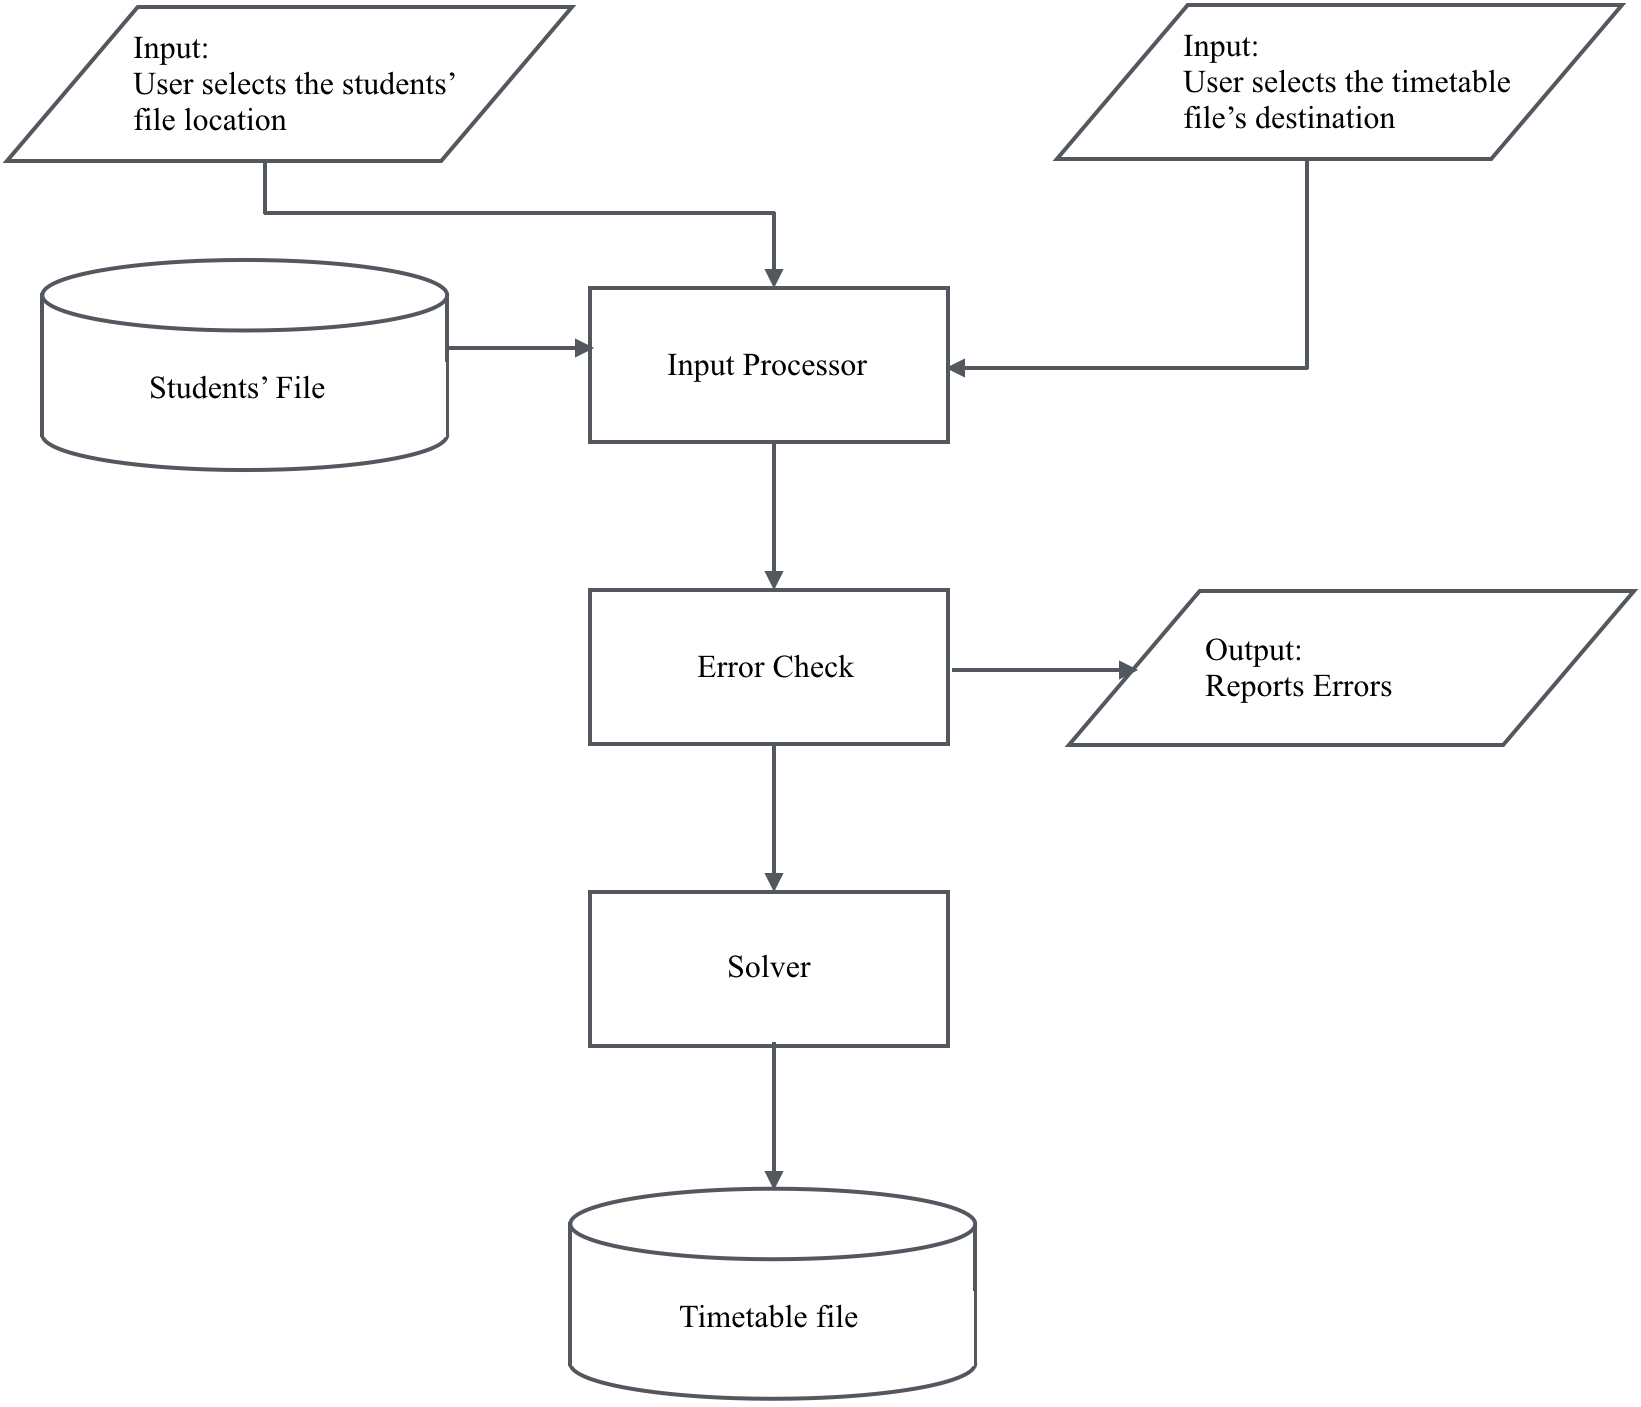
\includegraphics[width=\textwidth]{system_flowchart}
\end{figure}
%
\section{GUI}

This will be the GUI of the program. The user will first click on the \textbf{Open Students
File} button, at which point a file dialog will open for them to select the .xlsx file
containing the students. Then, they will click on \textbf{Generate \& Output Timetable} to
open a second file dialog to select the location and name of the file where the output of
the program will be stored. Finally, the \textbf{options} menu will contain any possible
options for the output, such as whether to also consider teachers' schedules when planning. 
%
\begin{figure}[H]
    \centering
    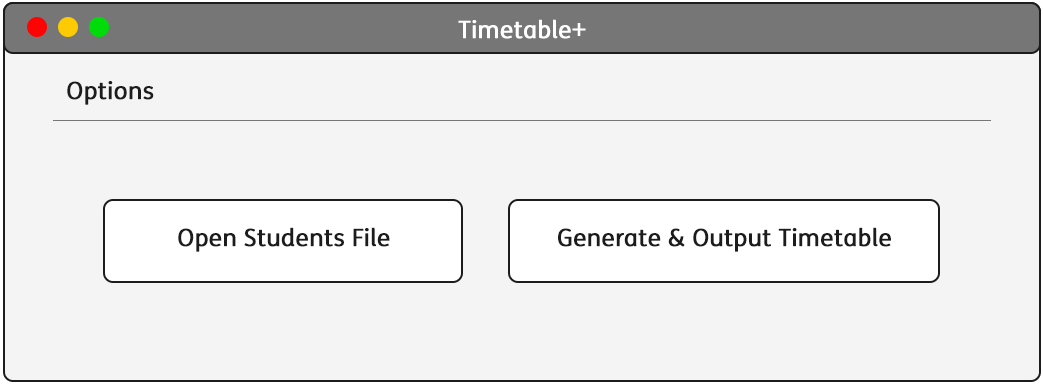
\includegraphics[width=\textwidth]{interface_design}
\end{figure}
%

\section{Module structure}

\begin{itemize}
    \item models.py
        \begin{itemize}
            \item class \texttt{Datastore}
            \item class \texttt{Subject}
        \end{itemize}
    \item views.py
        \begin{itemize}
            \item function \texttt{timetable\_to\_ascii\_table(timetable)}
            \item function \texttt{timetable\_to\_workbook(timetable, sheet\_name)}
        \end{itemize}
    \item interface.py
        \begin{itemize}
            \item class \texttt{MainWindow}
        \end{itemize}
    \item solver.py
        \begin{itemize}
            \item function \texttt{possible\_timetables(students, periods\_per\_week)}
        \end{itemize}
\end{itemize}

\subsection{Classes}
Methods surrounded by underscores (such as \_\_method\_name\_\_) are so-called python
\emph{magic methods} and are not called directly by my code but are instead used to give
more functionality to the classes. The \_\_eq\_\_(other) method, for example allows the
class that implements it to be compared with any other object using the \texttt{==} operator
in the way defined by the programmer.

%
\begin{table}[H]
    \centering
\begin{tabular}{|l r|}
    \hline
    \multicolumn{2}{|c|}{Datastore}\\
    \hline
    \hline
    openpyxl.worksheet.Worksheet & worksheet\\
    \hline
    Generator\footnotemark & getSubjects()\\
    Dict      & getStudents(includeTeachers)\\
    \hline
\end{tabular}
\end{table}
\footnotetext{to be explained in Development section}
%

%
\begin{table}[H]
    \centering
\begin{tabular}{|l r|}
    \hline
    \multicolumn{2}{|c|}{Subject}\\
    \hline
    \hline
    str & name\\
    int & periods\_per\_week\\
    str & teacher name\\
    \hline
    bool & \_\_eq\_\_(other)\\
    int  & \_\_hash\_\_()\\
    \hline
\end{tabular}
\end{table}
%


%
\begin{table}[H]
    \centering
\begin{tabular}{|l r|}
    \hline
    \multicolumn{2}{|c|}{MainWindow (Subclass of PyQt.QtWidgets.QMainWindow)}\\
    \hline
    \hline              
    & \\[-0.5em]
    \hline
    void & get\_file\_to\_open()\\
    void & generate\_timetable()\\
    \hline
\end{tabular}
\end{table}
%


\section{Input File structure}
This is the structure of the input file. Column A will be ignored, and is used for labels.
Then, each column corresponds to a class. The following rows contained data as per the
labels in column A. If row 4 is empty or 0, the no extra HL periods will be scheduled. 

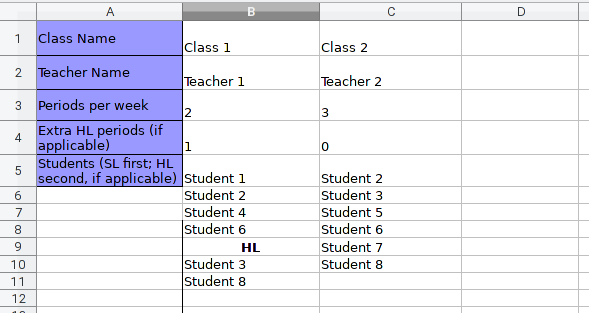
\includegraphics[width=\textwidth]{data_file_structure.png}

\section{Testing}

First I am going to test using valid data, namely the data for the class of 2018, to check
that
%
\begin{itemize}
    \item No student has two subjects scheduled to the same period
    \item All subjects are scheduled
    \item Each subject has the correct number of periods
    \item Subjects that have extra hl periods have had them scheduled
\end{itemize}
%

To make testing quicker, I will add functionality to the program to have make it output the
timetable directly on the command line. Therefore, after the rest of the testing, I will
also check the Excel output:
%
\begin{itemize}
    \item It can be opened with Microsoft Excel
    \item It is identical to the terminal output
\end{itemize}
%

Afterwards, I will also test using malformed data, to ensure that no invalid output is
produced. 
%
\begin{itemize}
    \item Empty file, should output an empty table
    \item Subject with no students, the subject should not be included in the output
    \item Subject name missing from one column, should output error message pointing to the
        cell where the name should be
    \item Number of periods missing for one subject, should output error message pointing to
        the cell where the number of periods should be
\end{itemize}
%


\end{document}
